\documentclass{memoir}
\usepackage{mystyle}

\begin{document}

\setcounter{section}{10}

\section{Direct Sums}

\begin{prp}
If $V$ and $W$ are $F$-vector spaces, then the set \[V \oplus W = \{(v,w) \mid v \in V, w \in W\}\] is an $F$ vector space with the operations \[ (v_1,w_1) + (v_2,w_2) = (v_1+v_2, w_1+w_2) \] and \[ \alpha(v,w) = (\alpha v, \alpha w). \] We call $V \oplus W$ the \emph{direct sum} of $V$ and $W$.
\end{prp}

\begin{prp} \mbox{}
\begin{enumerate*}
\item $V \oplus 0 \cong V$
\item $V \oplus W \cong W \oplus V$
\item $V \oplus (W \oplus U) \cong (V \oplus W) \oplus U$
\end{enumerate*}
\end{prp}

\begin{proof}
Exercise.
\end{proof}

\begin{prp}[Universal Property of $\oplus$, Part I] \mbox{}
\begin{enumerate*}
\item The projection maps $\pi_V : V \oplus W \rightarrow V$ and $\pi_W : V \oplus W \rightarrow W$ given by $\pi_V(v,w) = v$ and $\pi_W(v,w) = w$ are surjective linear transformations.
\item If $U$ is an $F$-vector space and $\varphi_V : U \rightarrow V$ and $\varphi_W : U \rightarrow W$ are linear transformations, then there is a unique linear transformation $\Theta : U \rightarrow V \oplus W$ such that $\varphi_V = \pi_V \circ \Theta$ and $\varphi_W = \pi_W \circ \Theta$. That is, there is a unique $\Theta$ such that the following diagram commutes.

\begin{center}
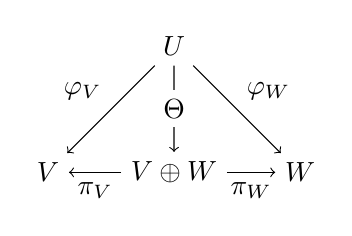
\begin{tikzpicture}[scale=0.8]
  \node (U) at (2,2) {$U$};
  \node (V) at (0,0) {$V$};
  \node (W) at (4,0) {$W$};
  \node (P) at (2,0) {$V \oplus W$};
  \draw[->] (U) edge node [above left] {$\varphi_V$} (V);
  \draw[->] (U) edge node [above right] {$\varphi_W$} (W);
  \draw[->] (P) edge node [below] {$\pi_V$} (V);
  \draw[->] (P) edge node [below] {$\pi_W$} (W);
  \draw[->] (U) edge node [style={fill=white}] {$\Theta$} (P);
\end{tikzpicture}
\end{center}
\end{enumerate*}
\end{prp}

\begin{proof} \mbox{}
\begin{enumerate*}
\item We have \[ \pi_V((v_1,w_1) + (v_2,w_2)) = \pi_V(v_1+v_2, w_1+w_2) = v_1+v_2 = \pi_V(v_1,w_1) + \pi_V(v_2,w_2) \] and \[ \pi_V(\alpha(v,w)) = \pi_V(\alpha v, \alpha w) = \alpha v = \alpha \pi_V(v,w), \] so $\pi_V$ is a linear transformation. Similarly for $\pi_W$.
\item Define $\Theta : U \rightarrow V \oplus W$ by $\Theta(u) = (\varphi_V(u), \varphi_W(u))$. Then \[ \begin{array}{ccc} \Theta(u_1 + u_2) & = & (\varphi_V(u_1+u_2), \varphi_W(u_1+u_2)) \\ & = & (\varphi_V(u_1) + \varphi_V(u_2), \varphi_W(u_1) + \varphi_W(u_2)) \\ & = & (\varphi_V(v_1), \varphi_W(u_1)) + (\varphi_V(u_2), \varphi_W(u_2)) \\ & = & \Theta(u_1) + \Theta(u_2) \end{array} \] and \[ \Theta(\alpha u) = (\varphi_V(\alpha u), \varphi_W(\alpha u)) = (\alpha\varphi_V(u), \alpha\varphi_W(u)) = \alpha(\varphi_V(u),\varphi_W(u)) = \alpha\Theta(u) \] so that $\Theta$ is linear. Moreover, \[ (\pi_V \circ \Theta)(u) = \pi_V(\Theta(u)) = \pi_V(\varphi_V(u), \varphi_W(u)) = \varphi_V(u) \] and similarly $\pi_W \circ \Theta = \varphi_W$, as claimed. Finally, if $\Psi : U \rightarrow V \oplus W$ is another linear transfomation having this property, then we can write $\Psi(u) = (\mu(u), \eta(u))$ for some functions $\mu$ and $\eta$. But then \[ \mu(u) = (\pi_V \circ \Psi)(u) = \varphi_V(u) \] and likewise $\eta = \varphi_W$, so in fact $\Psi = \Theta$. \qedhere
\end{enumerate*}
\end{proof}

\begin{prp}[Universal Property of $\oplus$, Part II] \mbox{}
\begin{enumerate*}
\item The injection maps $\iota_V : V \rightarrow V \oplus W$ and $\iota_W : W \rightarrow V \oplus W$ given by $\pi_V(v) = (v,0)$ and $\pi_W(w) = (0,w)$ are injective linear transformations.
\item If $U$ is an $F$-vector space and $\varphi_V : V \rightarrow U$ and $\varphi_W : W \rightarrow U$ are linear transformations, then there is a unique linear transformation $\Theta : V \oplus W \rightarrow U$ such that $\varphi_V = \Theta \circ \iota_V$ and $\varphi_W = \Theta \circ \iota_W$. That is, there is a unique $\Theta$ such that the following diagram commutes.

\begin{center}
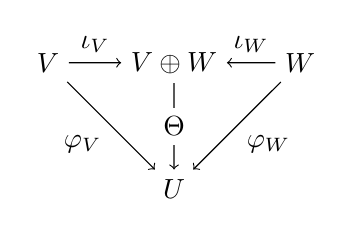
\begin{tikzpicture}[scale=0.8]
  \node (U) at (2,0) {$U$};
  \node (V) at (0,2) {$V$};
  \node (W) at (4,2) {$W$};
  \node (S) at (2,2) {$V \oplus W$};
  \draw[->] (V) edge node [below left] {$\varphi_V$} (U);
  \draw[->] (W) edge node [below right] {$\varphi_W$} (U);
  \draw[->] (V) edge node [above] {$\iota_V$} (S);
  \draw[->] (W) edge node [above] {$\iota_W$} (S);
  \draw[->] (S) edge node [style={fill=white}] {$\Theta$} (U);
\end{tikzpicture}
\end{center}
\end{enumerate*}
\end{prp}

\begin{proof}
Exercise.
\end{proof}

\begin{prp}
If $\mathcal{B} \subseteq V$ and $\mathcal{E} \subseteq W$ are bases, then $\mathcal{B} \oplus \mathcal{E} = (\mathcal{B} \times 0) \cup (0 \times \mathcal{E})$ is a basis of $V \oplus W$.
\end{prp}

\begin{proof}
Let $(v,w) \in V \oplus W$. Since $\mathcal{B}$ and $\mathcal{E}$ are bases, we have $v = \sum_{i=1}^m \alpha_i b_i$ and $w = \sum_{i=1}^n \beta_i e_i$ for some $\alpha_i,\beta_i \in F$, $b_i \in \mathcal{B}$, and $e_i \in \mathcal{E}$. Clearly then \[ (v,w) = \sum_{i=1}^m \alpha_i (b_i,0) + \sum_{i=1}^n \beta_i(0,e_i) \] so that $\mathcal{B} \oplus \mathcal{E}$ is a generating set for $V \oplus W$. Similarly, if \[ (0,0) = \sum_{i=1}^m \alpha_i (b_i,0) + \sum_{i=1}^n \beta_i(0,e_i) = \left(\sum_{i=1}^m \alpha_i b_i, \sum_{i=1}^n \beta_i e_i\right), \] then in fact $\alpha_i = \beta_i = 0$. Thus $\mathcal{B} \oplus \mathcal{E}$ is independent.
\end{proof}

\begin{cor}
If $V$ and $W$ are finite dimensional, then so is $V \oplus W$, and in fact \[ \Dim{V \oplus W} = \Dim{V} + \Dim{W}. \]
\end{cor}

If $\mathcal{B} = \{b_1,\ldots,b_m\}$ and $\mathcal{E} = \{e_1,\ldots,e_n\}$ are finite ordered bases, then we canonically order $\mathcal{B} \oplus \mathcal{E}$ as \[ \{ (b_1,0), \ldots, (b_m,0), (0,e_1), \ldots, (0,e_n) \}. \]

\begin{prp}
Suppose $\mathcal{B} \subseteq V$, $\mathcal{E} \subseteq W$, and $\mathcal{K} \subseteq U$ are (finite) bases.
\begin{enumerate*}
\item If $\varphi_V : U \rightarrow V$ and $\varphi_W : U \rightarrow W$ are linear transformations and $\Theta : U \rightarrow V \oplus W$ is the (unique) linear transformation given by the universal property of direct sums (part I), then \[ [\Theta]^\mathcal{K}_{\mathcal{B} \oplus \mathcal{E}} = \left[ \begin{array}{c} [\varphi_V]^\mathcal{K}_\mathcal{B} \\ \hline [\varphi_W]^\mathcal{K}_\mathcal{E} \end{array} \right]. \]
\item If $\varphi_V : V \rightarrow U$ and $\varphi_W : W \rightarrow U$ are linear transformations and $\Theta : V \oplus W \rightarrow U$ is the (unique) linear transformation given by the universal property of direct sums (part II), then \[ [\Theta]^{\mathcal{B} \oplus \mathcal{E}}_\mathcal{K} = \left[ \begin{array}{c|c} [\varphi_V]^\mathcal{B}_\mathcal{K} & [\varphi_W]^\mathcal{E}_\mathcal{K} \end{array} \right]. \]
\end{enumerate*}
\end{prp}

\subsection*{Direct Sums of Transformations}

\begin{dfn}
Suppose $\varphi_1 : V_1 \rightarrow W_1$ and $\varphi_2 : V_2 \rightarrow W_2$ are linear transformations. Then the mapping $\varphi_1 \oplus \varphi_2 : V_1 \oplus V_2 \rightarrow W_1 \oplus W_2$ given by \[ (\varphi_1 \oplus \varphi_2)(v_1,v_2) = (\varphi_1(v_1), \varphi_2(v_2)) \] is a linear transformation.
\end{dfn}

\begin{prp}
Suppose $\mathcal{B}_1 \subseteq V_1$, $\mathcal{B}_2 \subseteq V_2$, $\mathcal{E}_1 \subseteq W_1$, and $\mathcal{E}_2 \subseteq W_2$ are finite bases and that $\varphi_1 : V_1 \rightarrow W_1$ and $\varphi_ : V_2 \rightarrow W_2$ are linear transformations. If we define the \emph{block sum} of two matrices to be \[ A \oplus B = \left[ \begin{array}{c|c} A & 0 \\ \hline 0 & B \end{array} \right], \] then we have the pleasing equation \[ [\varphi_1 \oplus \varphi_2]^{\mathcal{B}_1 \oplus \mathcal{B}_2}_{\mathcal{E}_1 \oplus \mathcal{E}_2} = [\varphi_1]^{\mathcal{B}_1}_{\mathcal{E}_1} \oplus [\varphi_2]^{\mathcal{B}_2}_{\mathcal{E}_2}. \]
\end{prp}

\subsection*{Internal Direct Sums}

We can think of $\oplus$ as an operation which takes two vector spaces $V$ and $W$ and returns the smallest vector space containing disjoint copies of $V$ and $W$. Let's turn this problem around. Given a vector space $U$ together with two subspaces $V$ and $W$, when can we conclude that $U \cong V \oplus W$? Let us meditate on $\oplus$ for a moment. The direct sum $V \oplus W$ is a vector space having the following nice properties.
\begin{enumerate*}
\item $V \cong V \oplus 0$ and $W \cong 0 \oplus W$ are (isomorphic to) subspaces of $V \oplus W$.
\item $V + W = V \oplus W$ (rather, the isomorphic copies of $V$ and $W$)
\item $V \cap W = 0$ (again, the isomorphic copies)
\end{enumerate*}
Suppose we are given a big vector space $U$ together with two subspaces $V,W \subseteq U$ which have these properties. It turns out that this is exactly what is needed to show that $U \cong V \oplus W$.

\begin{prp}
Let $U$ be a vector space and let $V,W \subseteq U$ be subspaces. If $V + W = U$ and $V \cap W = 0$, then in fact $U \cong V \oplus W$ and we say that $U$ is the \emph{internal direct sum} of its subspaces $V$ and $W$.
\end{prp}

\begin{proof}
Exercise.
\end{proof}

Suppose $\varphi : V \rightarrow V$ is a linear transformation, with $V$ finite dimensional. Suppose further that we can find subspaces $W_1$ and $W_2$ such that $\varphi[W_1] \subseteq W_1$ and $\varphi[W_2] \subseteq W_2$ and $V$ is the internal direct sum of $W_1$ and $W_2$. Using 11.9, there is a suitable basis $\mathcal{B}$ for $V$ (namely, the union of bases for $W_1$ and $W_2$) such that the matrix of $\varphi$ has the form \[ \left[ \begin{array}{c|c} A & 0 \\ \hline 0 & B \end{array} \right], \] which has plenty of zeros and thus is in some sense ``preferable'' to one with fewer zeros. For example, the powers of such a matrix behave nicely: \[ \left[ \begin{array}{c|c} A & 0 \\ \hline 0 & B \end{array} \right]^k = \left[ \begin{array}{c|c} A^k & 0 \\ \hline 0 & B^k \end{array} \right]. \]

In a few days we will see that there is a general procedure for finding a ``best possible'' basis for $V$; one which makes the matrix of $\varphi$ have as many zeros as possible.

\end{document}